\begin{figure}[h]
    \centering
    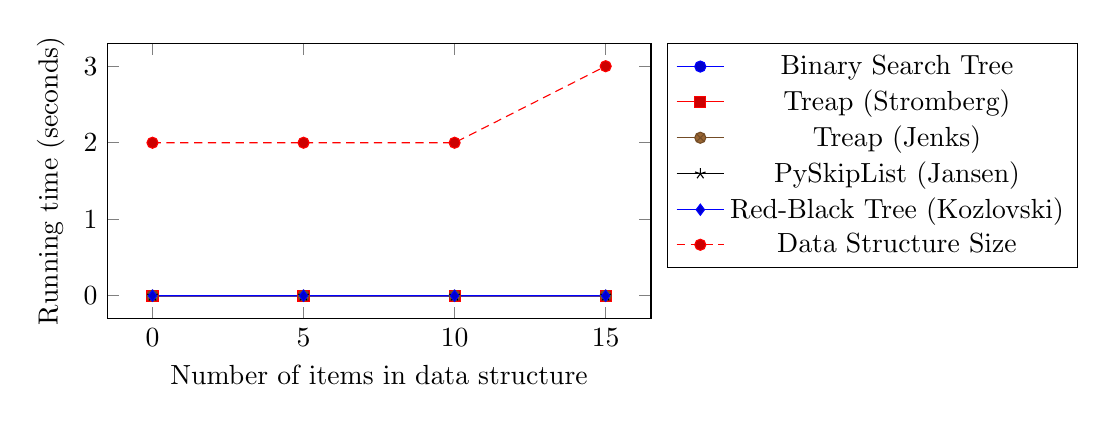
\begin{tikzpicture}
        \begin{axis}[
            xlabel={Number of items in data structure},
            ylabel={Running time (seconds)},
            title={},
            width=0.7\textwidth,
            height=2in,
            legend pos=outer north east
        ]
		\addplot coordinates {
			(0, 3.1121451464339277e-06)
			(5, 3.0117533675167647e-06)
			(10, 2.3090109150961913e-06)
			(15, 2.6101862518478243e-06)
		};
		\addplot coordinates {
			(0, 6.7262491874541036e-06)
			(5, 6.826640966371411e-06)
			(10, 2.6101862518479687e-06)
			(15, 4.015671156689116e-06)
		};
		\addplot coordinates {
			(0, 6.123898513950693e-06)
			(5, 5.722331398281752e-06)
			(10, 2.7105780307651317e-06)
			(15, 2.3090109150961913e-06)
		};
		\addplot coordinates {
			(0, 1.0139569670639809e-05)
			(5, 1.0139569670639809e-05)
			(10, 5.019588945861323e-06)
			(15, 1.1545054575480955e-05)
		};
		\addplot coordinates {
			(0, 8.131734092295395e-06)
			(5, 1.134427101764634e-05)
			(10, 7.5293834187918395e-06)
			(15, 2.9113615885994573e-06)
		};
		\addplot coordinates {
			(0, 2)
			(5, 2)
			(10, 2)
			(15, 3)
		};
        \legend{Binary Search Tree, Treap (Stromberg), Treap (Jenks), PySkipList (Jansen), Red-Black Tree (Kozlovski), Data Structure Size}
        \end{axis}
    \end{tikzpicture}
    \caption{Average of 3 operations, benchmarked every 5, starting at 0.}
\end{figure}